\section{Nonreciprocal behavior}

\begin{frame}{Performed tests}

    Both experimental and numerical simulations have shown that the structure exhibits a nonreciprocal behavior when excited with a time-space modulated signal.

    \begin{figure}[H]
        \centering
        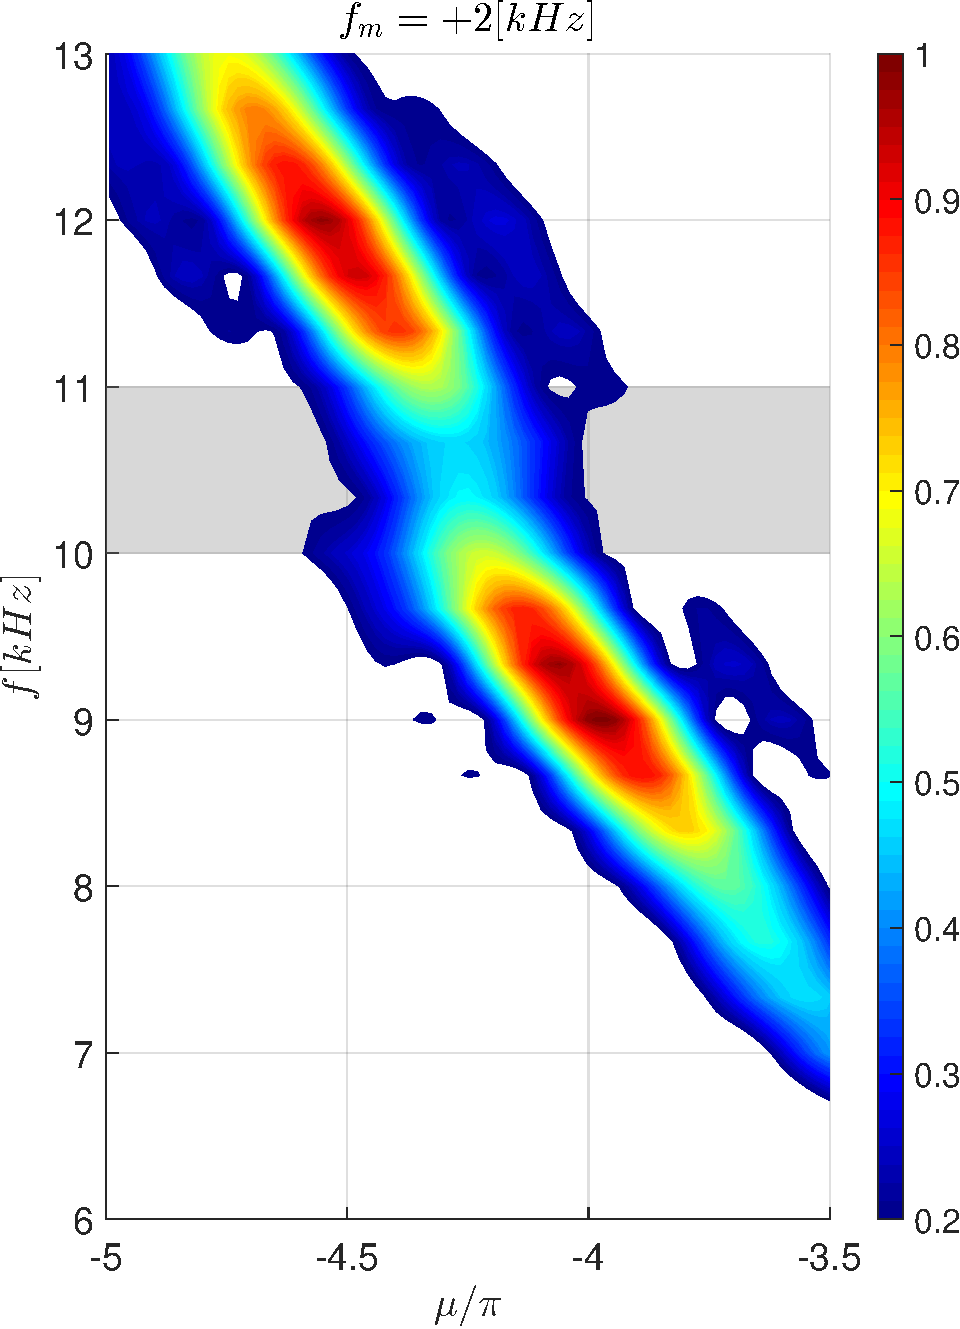
\includegraphics[width=0.3\textwidth]{img/MATLAB/EXP_nonreciprocal_@+2kHz.pdf}
        \hspace{1cm}
        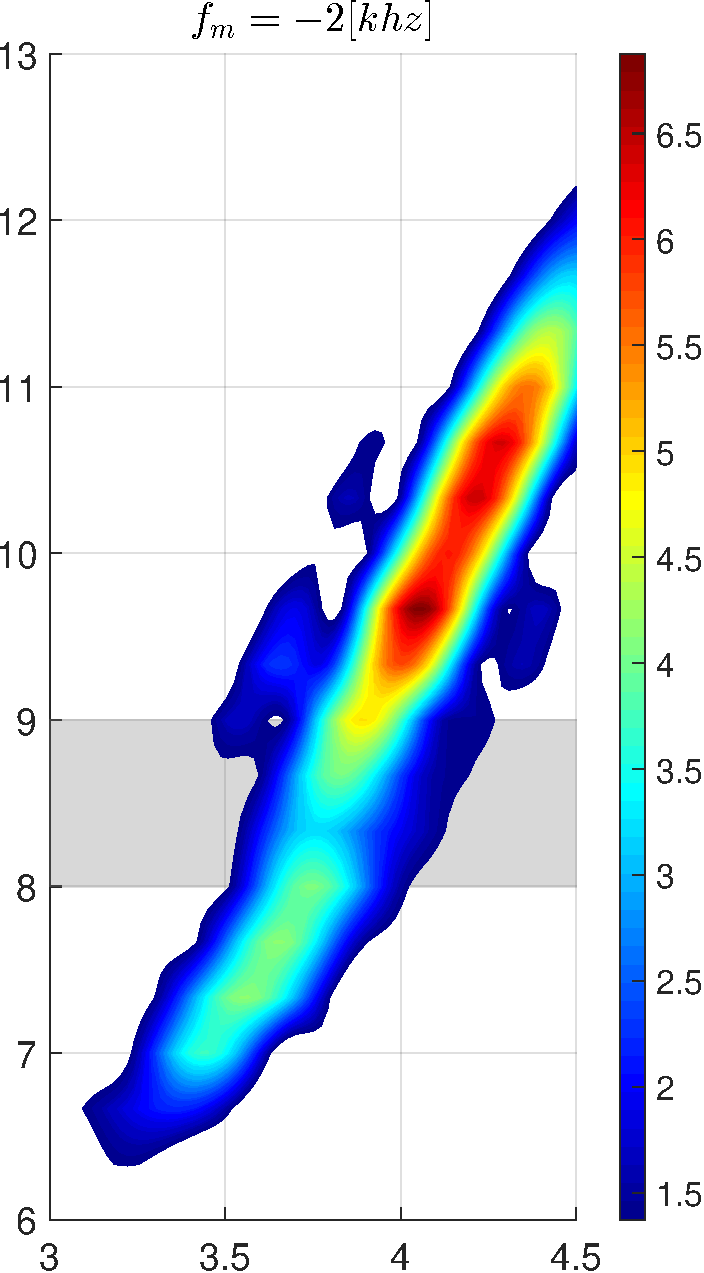
\includegraphics[width=0.3\textwidth]{img/MATLAB/EXP_nonreciprocal_@-2kHz.pdf}
        \caption{Experimental results for modulation frequency $f_m = \pm 2 kHz$.}
    \end{figure}

    Two additional tests are performed using a narrow-band excitation signal at the two directional band-gaps frequencies already identified.
    Spectral analysis of the travelling waves is performed to further highlight nonreciprocity in the structure.

\end{frame}



\begin{frame}{Spectral analysis}

    \begin{figure}[H]
        \centering
        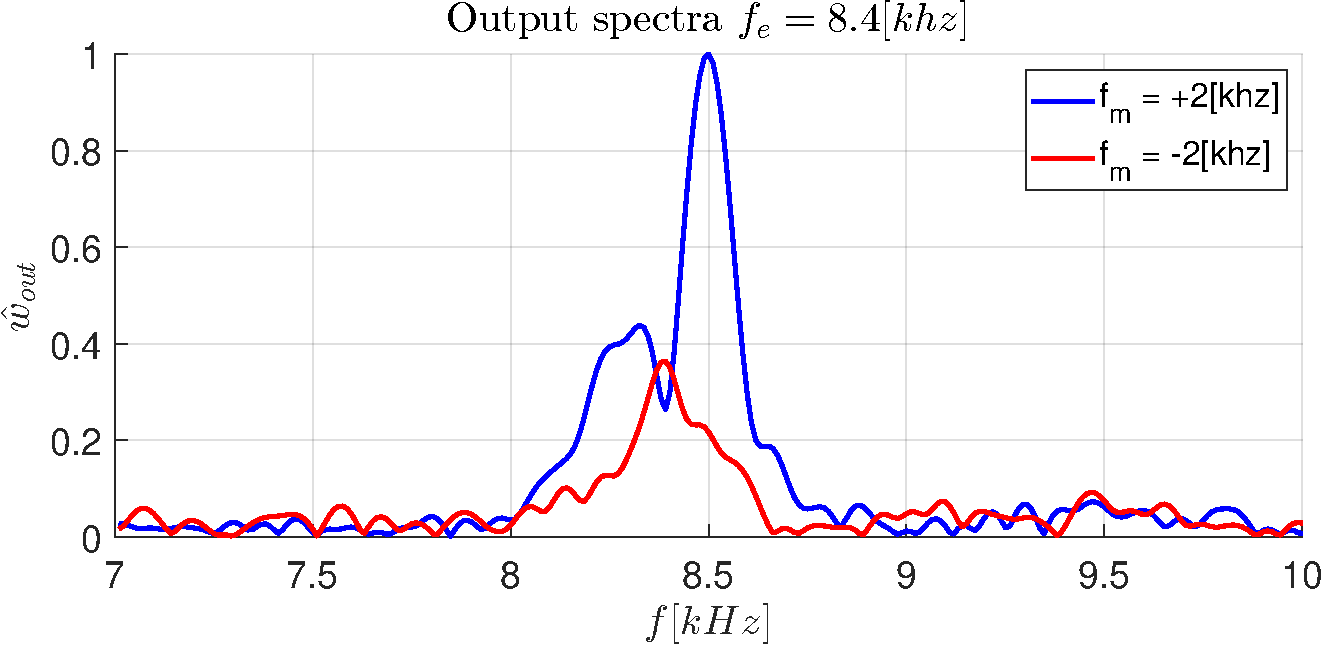
\includegraphics[width=0.49\textwidth]{img/MATLAB/Spectra_narrow8p4kHz_2000.pdf}
        \hfill
        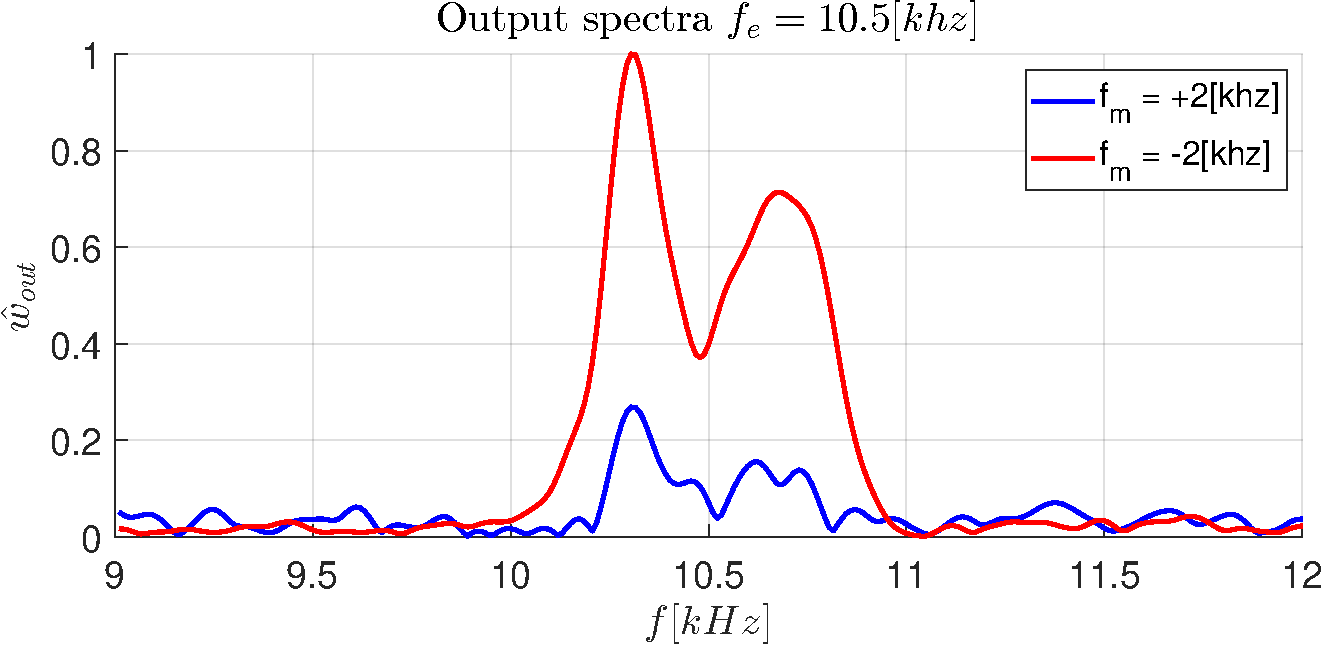
\includegraphics[width=0.49\textwidth]{img/MATLAB/Spectra_narrow10p5kHz_2000.pdf}
        \caption{Spectral components of end-of-beam displacement for (left) $f_e = 8.4 kHz$ and (right) $f_e = 10.5 kHz$ excitations. Modulation frequency is set to $f_m = \pm 2 kHz$.}
    \end{figure}

    \textbf{Depending on the travelling direction considered, the wave propagates differently.}
    The principle of reciprocity is therefore violated.

\end{frame}